% !TEX root = ./IQF - Slides Anotações.tex
% Slide 3 - Calorimetria e 1a Lei da Termodinâmica

\setcounter{part}{2}
\part{Calorimetria e 1\textsuperscript{a} Lei da Termodinâmica}

% Revisão aula passada
    % Diagrama de fases

    % Diagrama de fases: graus de liberdade
        % Quantidade de variáveis que posso variar para manter a situação
        % pode definir um ponto (GL0), uma curva (GL1) ou uma area (GL2)

% fim da revisão

\begin{sectionBox}1{Forças Intermoleculares}

    \begin{sectionBox}*2{Forças Eletrostáticas}
        \begin{BM}
                \text{Ião-Ião:}    &\quad E_p\propto(q_1\,q_2)/r
            \\  \text{Ião-Dipolo:} &\quad E_p\propto|z|\,\mu/r^2
        \end{BM}
    \end{sectionBox}

    \begin{sectionBox}*2{Forças de Van der Waals}
        \begin{BM}
                \text{Dipolo-Dipolo}
                &\quad
                    \begin{cases}
                        E_p\propto -(\mu_1^2\,\mu_2^2)/r^6  &\quad\ch{\gas}
                    \\  E_p\propto -(\mu_1\,\mu_2)/r^3      &\quad\ch{not \gas}
                    \end{cases}
            \\  \text{Dipolo-Dip. ind.}
                &\quad
                    E_p\propto-(\mu_1^2\,\alpha_2)/r^6
            \\  \text{Dip. ind. - Dip. Ind.}
                &\quad
                    E_p\propto-(\alpha_1\,\alpha_2)r^6
        \end{BM}
    \end{sectionBox}

\end{sectionBox}


\begin{sectionBox}1{Trabalho}
    \begin{BM}
        W
        =   \left(
                \begin{array}{c}
                    \text{Força contrária}
                \\  \text{ao movimento}
                \end{array}
            \right)
        \times
            \left(
                \begin{array}{c}
                    \text{Distancia}
                \\  \text{movimentada}
                \end{array}
            \right)
        \\
            [W] = \unit{\joule}
    \end{BM}

    \begin{sectionBox}*2{Trabalho de uma expansão}
        \begin{BM}
            W = -p_{\text{ext}}\,\adif{V}
        \end{BM}
    \end{sectionBox}

    \begin{sectionBox}*2{Trabalho de uma expansão isotérmica reversível}
        \begin{flalign*}
            &
                \odif{w}
            =   -p_{\text{ext}}\,\odif{v}
            =   -n\,R\,T\,\odif{v}/v
            =   -n\,R\,T\int_{v_i}^{v_f}\odif{v}/v
            =   -n\,R\,T\,\ln(v_f/v_i)
            &
        \end{flalign*}
    \end{sectionBox}

\end{sectionBox}


\begin{sectionBox}1{Calor}

    A energia interna do sistema, sua capacidade de realizar trabalho, pode ser variada pela troca de energia de e para sua vizinhança como calor quando há diferentes temperaturas dentre os corpos envolvidos.

    \begin{BM}
        q = C_{s}\,m\,\adif{T}
    \end{BM}

    \paragraph{obs:} \( 1\,\unit{\calorie} = 4.184\,\unit{\joule} \) (exatamente)

    \begin{sectionBox}*2{Capacidade calorifica}
        \begin{BM}
            c
            =   \frac{\text{calor fornecido}}{\text{variação de temperatura}}
            =   q/\adif{T}
        \end{BM}

        \begin{itemize}
            \item \(C_s = C/m\phantom{n}\)\quad capacidade calorífica específica
            \item \(C_n = C/n\phantom{m}\)\quad capacidade calorífica molar
        \end{itemize}

    \end{sectionBox}

\end{sectionBox}

\begin{sectionBox}1{1\textsuperscript{a} Lei da termodinâmica}

    
    \begin{BM}
        U \coloneqq Q+W
    \end{BM}

    Lei da conservação de energia.

    \begin{itemize}
        \item[\textit{Q}:] Calor
        \item[\textit{W}:] Trabalho
    \end{itemize}

    \begin{sectionBox}*2{\textit{U} é uma função de estado}

        \begin{BM}
            \Delta U = U_f - U_i
        \end{BM}

        independe do caminho percorrido.

    \end{sectionBox}

\end{sectionBox}


\begin{sectionBox}1{Energia interna de um gás}

    \begin{BM}
        E_i = -k\,T/2 \qquad k=1.381*10^{-23}\,\unit{\joule\per\kelvin}
    \end{BM}

    % \( k=1.381*10^{-23}\,\unit{\joule\per\kelvin} \)

    \begin{sectionBox}*2{Energia cinética de um átomo}
        \begin{BM}
            E_k = \frac{m}{2}\sum_{k=1}^{3}v_k^2\quad:v\in\mathbb{R}^3
        \end{BM}
    \end{sectionBox}

\end{sectionBox}


\begin{sectionBox}1m{Entalpia}

    \begin{BM}
        H \coloneqq U + P\,V
    \end{BM}

    \begin{itemize}
        \item[\textit{U}:] Energia interna do sistema
        \item[\textit{P}:] Pressão do sistema
        \item[\textit{V}:] Volume do sistema
    \end{itemize}

    \paragraph{Obs:} Pode-se ver que a entalpia é uma função de estado por suas componentes \textit{U}, \textit{P} e \textit{V} tambem serem

    \begin{sectionBox}*2{Transferencia de calor a pressão constante}
            
        \begin{BM}
            \Delta H = Q 
            :   \begin{cases}
                    \Delta P = 0
                \\  W = -P_{\text{ext}}\,\Delta V
                \\  P = P_{\text{ext}}
                \end{cases}
        \end{BM}
    
        \begin{flalign*}
            &
                \begin{array}{ll}
                    & \Delta H = \Delta U + P\,\Delta V
                \,\land\\\land &
                    \Delta U = Q+W
                \,\land\\\land &
                    W = -P_{\text{ext}}\,\Delta V
                \,\land\\\land &
                    P_{\text{ext}} = P
                \end{array}
            \implies &\\& \implies
                \Delta H = Q -P\,\Delta V+P\,\Delta V = Q
            &
        \end{flalign*}
        
    \end{sectionBox}

\end{sectionBox}

\begin{sectionBox}2m{Entalpia de transformações físicas}

    \begin{sectionBox}*3{Vaporização}
        \begin{BM}
            \Delta H_{\text{vap}}
        =   \Delta H_m(\text{vapor})
        -   \Delta H_m(\text{liquido})
        \end{BM}
    \end{sectionBox}
    
    \begin{sectionBox}*3{Entalpia de Fusão}
        \begin{BM}
            \Delta H_{\text{fus}}
        =   \Delta H_{m}(\text{liquido})
        -   \Delta H_{m}(\text{sólido})
        \end{BM}
    \end{sectionBox}
    
    \begin{sectionBox}*3{Entalpia de Sublimação}
        \begin{BM}
            \Delta H_{\text{sub}}
        =   \Delta H_{m}
        \end{BM}
    \end{sectionBox}

    \begin{sectionBox}*3{Curvas de aquecimento}

        % TODO: replace figures with actual graphs
        \begin{figure}[H]\centering
            
            % \begin{subfigure}{width=.9\linewidth}
                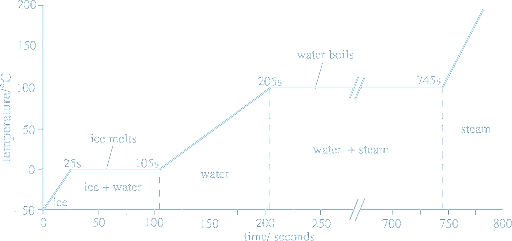
\includegraphics[width=.9\linewidth]{IQF - Slide 4 curva de aquecimento 1.png}
                \caption{Curva de aqueçimento de água (substancia pura)}
            % \end{subfigure}
            
            % \begin{subfigure}{width=.9\linewidth}
            %         \includegraphics[width=.9\textwidth]{resources/IQF - Slide 4 curva de aquecimento 2.png}
            % \end{subfigure}
            
        \end{figure}

        \begin{enumerate}
            \item Temperatura constante durante mudanças de fase
        \end{enumerate}

    \end{sectionBox}

\end{sectionBox}

\begin{sectionBox}2m{Entalpia de uma transformação química}

    \begin{itemize}
        \item Entalpia de reação
        \item Entalpia de reação padrão
        \item Entalpia de combustão padrão
        \item Entalpia de formação padrão
    \end{itemize}

    \begin{sectionBox}*3{Entalpia de formação padrão}
        \begin{BM}
            \Delta H_r^{\circ}
        =   \sum^n\,\Delta H_{f,(produtos)\,i}^{\circ}
        -   \sum^m\,\Delta H_{f,(reagentes)\,i}^{\circ}
        \end{BM}
    \end{sectionBox}

% % \tcbbreak
\end{sectionBox}
% \begin{sectionBox}m{}

\begin{questionBox}1m{}

    Ultilize a tabela a baixo para resolver as questões seguintes

    \begin{table}[H]\centering
        \begin{tabular}{c r r r}

            \toprule

            &   \multicolumn{1}{c}{\ch{C8H18\lqd{}}}
            &   \multicolumn{1}{c}{\ch{CO2\gas{}}}
            &   \multicolumn{1}{c}{\ch{H2O\gas{}}}

            \\\midrule

                \(\Delta H_f^{\circ}\) / \unit{\kilo\joule\per\mole}
            &   -249.9
            &   -393.5
            &   -241.8

            \\\bottomrule

        \end{tabular}
    \end{table}

    \begin{questionBox}2{}

        Equação de combustão do octano.

        \begin{center}
            \ch{C8H18\lqd{} + 25/2 O2 -> 8 CO2 + 9 H2O}
        \end{center}

    \end{questionBox}

    \begin{questionBox}2{}
        Calcule a entalpia padrão de combustão, \(\Delta H_c^{\circ}\), do octano.

        \begin{flalign*}
            &
                \Delta H_c^{\circ}
            = &\\&
            =   \left(
                -249.9
                -   (
                        8*(-393.5)
                    +   9*(-241.8)
                    )
                \right)
            \,  \unit{\kilo\joule\per\mole\of{\ch{C8H18\lqd{}}}}
            = &\\&
            =   5074.3\,\unit{\kilo\joule\per\mole\of{\ch{C8H18\lqd{}}}}
            &
        \end{flalign*}
    \end{questionBox}

% \end{questionBox}

% \end{sectionBox}
% \begin{sectionBox}m{}

% \begin{questionBox}m{}

    \begin{questionBox}2{}
        Calcule a variação de energia interna, \(\Delta U^{\circ}\), do sistema.
        \sisetup{
            round-precision = 5,
            round-mode      = figures
        }
        \begin{flalign*}
            &
                \Delta U
            =   q
            =   5074.3\,\unit{\kilo\joule\per\mole\of{\ch{C8H18\lqd{}}}}
            \,  \frac
                    {\unit{\calorie}}
                    {4.1868\,\unit{\joule}}
            \cong &\\&
            \cong
                \qty{1211.9757332569}{\kilo\calorie\per\mole\of{\ch{C8H18\lqd{}}}}
            &
        \end{flalign*}
    \end{questionBox}

    \begin{questionBox}2{}
        Quantos litros de água poderá usar no seu banho de imersão se puder usar o calor libertado na combustão acima para aquecer água cuja temperatura inicial seja 15\,\unit{celsius}? (Atenção: a temperatura do banho é escolhida por si e admita que não há percas de calor) Dados: \(\rho_{\ch{H2O\lqd{}}} = 1.00\,\unit{\gram\centi\meter^{-3}}; C_{p\,\ch{H2O\lqd{}}} = 4.2\,\unit{\joule\per{\kelvin\gram}}\).

        \begin{flalign*}
            &
                \text{Vol}_{\ch{H2O\lqd{}}}
            =   \frac
                    {\unit{\cubic{\centi\meter}\of{\ch{H2O\lqd{}}}}}
                    {1.00\unit{\gram\of{\ch{H2O\lqd{}}}}}
            \,  \frac
                    {\unit{\kelvin\gram\of{\ch{H2O\lqd{}}}}}
                    {4.2\,\unit{\joule}}
            \,  \frac
                    {5074.3\,\unit{\kilo\joule}}
                    {\unit{\mole\of{\ch{C8H18\lqd{}}}}}
            /   (35-15)\,\unit{\kelvin}
            \cong &\\&
            \cong
                \qty {60.408333333333333}
                    {\cubic{\centi\meter}\of{\ch{H2O\lqd{}}}\per\mole\of{\ch{C8H18\lqd{}}}}
            &
        \end{flalign*}
    \end{questionBox}

\end{questionBox}

% \end{sectionBox}
% \begin{sectionBox}m{}

% Q2
\begin{questionBox}1m{}
    Calcule a entalpia da reação de formação do cloreto de alumínio anidro

    \begin{center}
        \ch{2 Al\sld{} + 3 Cl2\gas{} -> 2 AlCl3\sld{}}
    \end{center}

    A partir dos seguintes dados

    \setlength\tabcolsep{0.2em}
    \begin{table}[H]\centering
        \begin{tabular}{c r}

            \toprule

                \multicolumn{1}{c}{Reação}
            &   \multicolumn{1}{c}{\(\Delta H_r^{\circ} / \unit{\kilo\joule\per\mole}\)}

            \\ \midrule

                \ch{2 Al\sld{} + 6 HCl\aq{} -> 2 AlCl3\aq{} + 3 H2\gas}
            &   -1049
            \\  \ch{HCl\gas{} -> HCl\aq{}}
            &   -74.8
            \\  \ch{H2\gas{} + Cl2\gas{} -> 2 HCl\gas{}}
            &   -185
            \\  \ch{AlCl3\sld{} -> AlCl3\aq{}}
            &   -323

            \\ \bottomrule

        \end{tabular}
    \end{table}

    \begin{center}
        \ch{
            Al\sld{} + 3/2 Cl2\gas{}
        ->  Al\sld{} + 3 HCl\gas{} - 3/2 H2\gas{}
        ->  Al\sld{} + 3 HCl\aq{} - 3/2 H2\gas{}
        ->  AlCl3\aq{}
        ->  AlCl3\sld{}
        }
    \end{center}

    \begin{flalign*}
        &
            \Delta H^{\circ}_{f\,\ch{AlCl3}}
        % = &\\&
        =   \left(
                1.5\,(-185)
            +   3\,(-74.8)
            +   0.5\,(-1049)
            -   (-323)
            \right)
        \,  \unit{\kilo\joule\per\mole\of{AlCl3\sld{}}}
        = &\\&
        =   -703.4\,\unit{\kilo\joule\per\mole\of{AlCl3\sld{}}}
        &
    \end{flalign*}

\end{questionBox}

% \end{sectionBox}





% % Exercício titulação (não faz parte da aula)
% \begin{sectionBox}{}
%
%     \begin{flalign*}
%         &
%             v\,\unit{\litre\of{\ch{HCl_{sol.i}}}}
%         =
%         \,  \frac
%                 {\unit{\litre\of{\ch{HCl_{sol.i}}}}}
%                 {1.189\,\unit{\kilo\gram\of{\ch{HCl_{sol.i}}}}}
%         \,  \frac
%                 {      \unit{\gram\of{\ch{HCl_{sol.i}}}}}
%                 {0.38\,\unit{\gram\of{\ch{HCl}}}}
%         \,  \frac
%                 {36.46\,\unit{\gram\of{\ch{HCl}}}}
%                 {       \unit{\mole\of{\ch{HCl}}}}
%         \,  \frac
%                 {0.39\,\unit{\mole\of{\ch{HCl}}}}
%                 {      \unit{\litre\of{\ch{HCl_{sol.f}}}}}
%         \,  250\,\unit{\milli\litre\of{\ch{HCl_{sol.f}}}}
%         \cong &\\&
%         \cong \qty{7.867845602230977}{\milli\litre\of{\ch{HCl_{sol.f}}}}
%         &
%     \end{flalign*}
%
% \end{sectionBox}
